\chapter{Física de semiconductores}

\section{Banda de valencia y conducción}

Un semiconductor es un material sólido que presenta dos bandas (en realidad presenta más, solo accesibles\footnote{Cuando decimos accesibles nos referimos a que existe una posibilidad no nula de que estén ocupadas.} a energías térmicas o electromagnéticas muy altas, y por tanto innecsarias para nuestro estudio). Para definir una banda primero tenemos que entender que los electrones en los sólidos se pueden describir mediante una suma de ondas planas, y por tanto la energía de estos se puede describir como una función del momento dse onda $E(k)$ (aunque no tiene porque ser necesariamente de la forma $E=\hbar^2 k^2/2m$). Así, debido al caracter fermiónico de los electrones y otros potenciales aparecen energías inaccesibles para nuestros electrones, i.e. para ningún $k$ existen esas energías. Así aparecen diferentes \textit{bandas}, limitadas por una \textit{energía superior} y una \textit{energía inferior}.

\begin{figure}[h!] \centering
	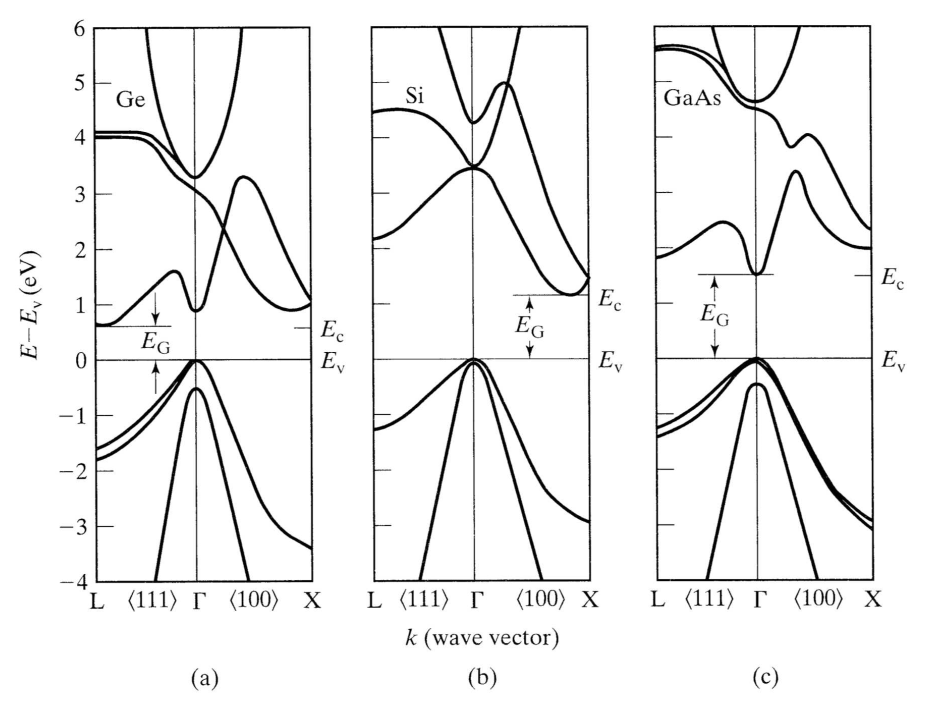
\includegraphics[width=0.7\textwidth]{Cuerpo/Ch_01/01_01.png}
	\caption{Bandas de conducción y valencia para algunos semicdonductores.}
\end{figure}

Como dijimos, un semiconductor posee dos bandas, separadas por una energía $E_g$. A la banda con energía superior se le llama \textbf{banda de conducción} (B.C) y a la banda inferior se le llama \textbf{banda de valencia} (B.V). Las bandas, a su vez, poseen diferentes líneas de dispersión, esto es diferentes relaciones $E(k)$. El número y forma de estas dependerá del tipo de material y la dirección de la onda, por esa misma razón solemos ver en la parte inferior de las bandas $\langle 111\rangle $ o $\langle 100\rangle$. Está denotando la dirección de la onda. En general suelen ser materiales muy simétricos, y por tanto con pocas direcciones representamos todas las posibles relacioens de dispersión.

La \textit{energía mínima de la banda de conducción} se denota como $E_c$, la \textit{energía máxima de la banda de valencia} se denota por $E_v$, y la diferencia entre el máximo de la BV y el mínimo de BC se denota por $E_g$:

\begin{equation}
	E_g = E_c - E_v
\end{equation}
En general se suele definir $E_v=0$ como referencia. Así la banda de valencia posee energías negativas, y la banda de conducción energías positivas. Veamos las características de las bandas:

\begin{itemize}
	\item \textbf{Banda de valencia:} el \textit{máximo siempre aparece en $k=0$}. Está dividida en 3 subbandas (3 relaciones de dispersión), 2 de ellas degeneradas en $k=0$ (son indistiguibles en $k=0$).
	\item \textbf{Banda de conducción:} está dividida en subbandas (aunque el número depende del material), y el valor de $k_{\min}$ tal que $E_{\min}=E(k_{\min})$ del dependerá del material.
\end{itemize}


\subsection{Semiconductores directos e indirectos}

Como hemos dicho, $E_c$ es el mínimo de la banda de conducción y $E_v$ es el máximo de la banda de valencia. En función del valor de $k_{\min}$ distinguimos dos tipos de semiconductores:
\begin{itemize}
	\item Definimos un \textbf{semiconductor indirecto} a aquel que verifica que $k_{\min}\neq0$. Es decir, el gap de energía sucede entre diferentes momentos (lo que hará que cuando se excite a un electrón de la BV tenga que darsele un momento).
	\item Definimos un \textbf{semiconductor directo} a aquel que verifica que $k_{\min}=0$. Es decir, el gap de energía sucede a $\Delta k =0$ (lo que hará que cuando se excite a un electrón de la BV no se pueda intercambiar momento).
\end{itemize}


\begin{figure}[h!] \centering
	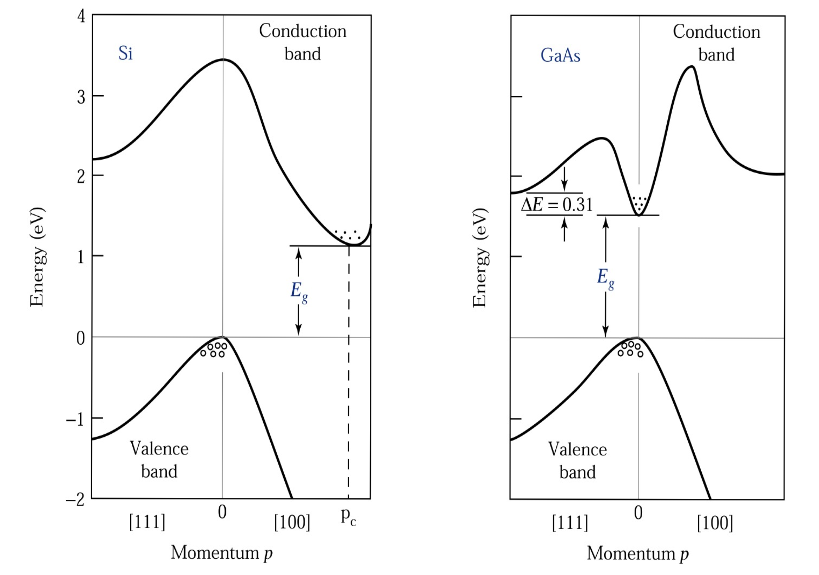
\includegraphics[width=0.8\textwidth]{Cuerpo/Ch_01/01_02.png}
	\caption{A la izquierda semicondutor de gap indirecto y a la derecha de gap directo.}
\end{figure}


\subsection{Forma de los mínimos y máximos de banda: masa equivalente}

Cerca de los extremos de las bandas $E_0=E(k_0)$ tenemos que se puede aproximar la enerǵia por una función parabólica, tal que:

\begin{equation}
	E = E_0 + \frac{1}{2} \parentesis{\parciales{^2E}{k^2}}_{k_0} (k-k_0)^2
\end{equation}
Como podemos ver, esto se parece mucho a la expresión $E=\hbar^2k^2/2m$ que se usa para \textit{partículas libres}. Es decir, cerca de los extremos de las bandas, los \textit{portadores actúan como partículas libres con masa efectiva $m^*$} definida como

\begin{equation}
	(m^*)^{-1} = \frac{1}{\hbar^2} \parciales{^2E}{k^2}
\end{equation}

\begin{Anotacion}
	\textcolor{red}{Imagen de los mínimos/máximos.}
\end{Anotacion}

\subsection{Ecuación del movimiento}

La ecuación del movimiento para los electrones es una generalización de la ecuación de Newton usando el momento de onda del electrón $\kn$. Sabiendo que

\begin{equation}
	\Fn = m^* \an = m^* \dot{\vn} = \dot{\pn} = \hbar\dot{\kn}
\end{equation}
de lo que se deduce que

\begin{equation}
	\hbar \derivadas{\kn}{t} = \Fn
\end{equation}
pudiendo ser la fuerza, por ejemplo, la fuerza de Lorentz $\Fn=-e(\En+\vn \times \Bn)$, o cualquier otra.

%%%%%%%%%%%%%%%%%%%%%%%%%%%%%%%%%%%%%%%%%%%%%%%%%%%%%%%%%%%%%%%%%%%%%%%
%%%%%%%%%%%%%%%%%%%%%%%%  SECCIÓN 2 %%%%%%%%%%%%%%%%%%%%%%%%%%%%%%%%%%%
%%%%%%%%%%%%%%%%%%%%%%%%%%%%%%%%%%%%%%%%%%%%%%%%%%%%%%%%%%%%%%%%%%%%%%%
\section{Portadores: conecpto de hueco y electrón}

En los semiconductores hay 2 tipos de portadores, los portadores tipo hueco (o tipo $p$\footnote{Por el hecho de que se pueden describir como partículas con carga positiva.}) y tipo electrón (tipo $n$). La pregunta que nos deberíamos plantear en este momento es: ¿Qué sentido tiene que existan portadores tipo electrón/hueco si solo tenemos electrones en el semiconductor?¿Como que ``tipo electrón'', no deberían ser simplemente electrones? La respuesta es un tanto complicada. Como hemos dicho, cerca de los extremos las partículas, los electrones se comportan como electrones libres con masa efectiva $m^*$ (de hay viene \textit{tipo electrón} se comportan casi como electrones). Sin embargo esta ``masa efectiva'' tiene un problema en el máximo de la banda de valencia: la masa efectiva es negativa (recordemos que en un máximo la curvatura $\partial^2 E/ \partial k^2<0$). 

Para solucionarlo trabajemos en la siguiente idea. Supongamos que tenemos la capa de valencia llena salvo por un electrón, que se ha excitado y ha subido a la capa de conducción. En la banda de valencia habrá entonces $N$ electrones menos uno. La suma de los momentos de todos los electrones de la banda será entonces:

\begin{equation}
	\kn = \sum_{i=1}^{4N-1} \kn_i
\end{equation}
o lo que es lo mismo:

\begin{equation}
	\kn = \sum_{i=1}^{4N} (\kn_i) - \kn_e
\end{equation}
denotándolo por $\kn_e$ ya que es un electrón cualquiera (son indistiguibles). Como sabemos, la suma del momento de los electrones en una banda tiene que ser cero, ya que $k$ tiene tanto valores negativos y positivas, y están todos ocupados. Es decir, tenemos que el momento total de la banda será:

\begin{equation}
	\kn \equiv \kn_h = - \kn_e
\end{equation}
si a este momento total lo llamamos $\kn_p$ (momento de portador $p$ o hueco), tenemos que \textit{el movimiento efectivo de una capa sin un electrón es en el sentido opuesto al que tendría un electŕon individual en la misma}. A este artificio matemático lo llamamos hueco, y no es más que la manera de describir el comportamiento de una capa entera (capa de valencia) a través de unas pocas partículas. La energía también tendrá el signo opuesto, ya que:

\begin{equation}
	E_h = \sum_{i} E_i - E_e
\end{equation}
y como $\sum_{i}E_i$ es una constante, la podemos ignorar. Así pues, definimos la \textit{energía del hueco}

\begin{equation}
	E_h \equiv - E_e
\end{equation}
Y por tanto, aunque la masa efectiva de un electrón en el máximo de la banda de valencia sea negativa (en un máximo $\partial^2 E/ \partial k^2<0$), para el objeto matemático así definido tenemos que la masa efectiva será positiva, y la carga será positiva. Que la carga sea positiva no es tan obvio. Para ello tenemos que ver que la ecuación del movimiento

\begin{equation}
	\hbar \derivadas{\kn_h}{t} = -e(\En + \vn_h \times \Bn)
\end{equation}
hace que se comporte como un electrón con carga positiva $(\kn_h \equiv - \kn_e)$. 

La pregunta ahora es: ¿Tiene sentido físico? La respuesta es que sí. El sentido físico está en que cuando excitamos un electrón a la BC desde la BV, queda un estado sin ocupar, un hueco, en la banda de valencia. Este hueco podría ser rellenado por los electrones vecinos, que desde fuera lo veríamos como un movimiento efectivo del hueco, que además tendría el sentido contrario al del electrón (si los electrones saltan por ejemplo de izquierda a derecha por culpa de un campo eléctrico, veremos al hueco saltando de la derecha a la izquierda).

Consecuentemente los electrones en la banda de conducción se comportarán como electrones normales libres por la salvedad de que la masa efectiva será diferente; mientras que la falta de electrones en la banda de valencia (por la excitación de estos a la banda de conducción) se describirá a través de una serie de partículas con masa efectiva positiva diferente a la masa del electrón, carga positiva, con momento y energía efectiva de signo contrario al que tendría un electrón libre en la banda de valencia.


%%%%%%%%%%%%%%%%%%%%%%%%%%%%%%%%%%%%%%%%%%%%%%%%%%%%%%%%%%%%%%%%%%%%%%%
%%%%%%%%%%%%%%%%%%%%%%%%  SECCIÓN 3 %%%%%%%%%%%%%%%%%%%%%%%%%%%%%%%%%%%
%%%%%%%%%%%%%%%%%%%%%%%%%%%%%%%%%%%%%%%%%%%%%%%%%%%%%%%%%%%%%%%%%%%%%%%

\section{Densidad de portadores y clasificación de semiconductores}

En esta sección vamos a tratar de expresar la densidad de portadores hueco, denotado por $p$, y la densidad de portadores electrones, denotado por $n$. Primero estudiaremos el caso mas general posible, en función de la densidad de estados $g(E)$ y de la función de Fermi-Dirac $f(E)$. Luego iremos haciendo ciertas aproximaciones para simplificar los resultados.

\subsection{Densidad de portadores en el caso más general posible}

El caso más general, como ya hemos dicho, estudia el número de portadores $n$ y $p$ a partir de las integrales sobre las densidades de energía y función de Fermi. La \textit{densidad de estados} $g(E)$ es la distribución de los estados de energía a una energía dada, mientras que la \textit{función de Fermi} indica, en condiciones de equlibrio, la probabilidad de que un estado permitido de enerǵia $E$ esté ocupado por un electrón. La función de densidad de estados depende de la dimensión del sistema, tal que:

\begin{equation}
	g_{3D} (E) = \frac{\sqrt{2}m^{3/2}E^{1/2}}{\pi^2 \hbar^3} \quad g_{2D} (E) = \frac{m}{\pi \hbar^2} \quad g_{1D} (E) = \frac{\sqrt{2}m^{1/2}}{\pi \hbar \sqrt{E}}
\end{equation}
La dedución de estas densidades no es exageradamente complicada, véase apéndice \ref{Sec:A-01}. Por otra parte, la función de Fermi nos dice que la probabilidad de que cierto estado esté ocupado es:


\begin{equation}
	f(E) = \frac{1}{1+e^{(E-E_F)/kT}}
\end{equation}
donde $E_F$ es la enerǵia de Fermi, de la cual hablaremos más adelante. Naifmente uno podría pensar que la densidad $n/p$ sería simplemente la integral $g(E)f(E)$ entre diferentes intervalos de energía, ya que como sabemos los electrones se encuentran siempre en la banda de conducción, y por tanto entre las energías $E_{\min}$ y $E_c$, mientras que los huecos se encuentran en la banda de valencia, y por tanto entre las energías $E_{\max}$ y $E_v$.

Sin embargo esto no es correcto, por dos razones. La primera de ellas es que por culpa de la forma de parábola cerca del máximo y el mínimo de la banda de valencia y conducción respectivamente, es necesario redefinir el cero en el máximo local/mínimo local. La razón no es evidente a primera vista, pero uno lo puede entender cuando piensa que en un extremo local solo caben 2 electrones (uno con espín arriba y otro con espín abajo). Así pues, las densidades en la banda de valencia $g_v(E)$ y en la banda de conducción $g_c(E)$ son:

\begin{equation}
	g_c(E) = \frac{(m_n^*)^{3/2} \sqrt{2(E-E_c)}}{\pi^2 \hbar^3} \quad E \geq E_c \qquad 	g_v(E) = \frac{(m_p^*)^{3/2} \sqrt{2(E_v-E)}}{\pi^2 \hbar^3} \quad E \leq E_v
\end{equation}
La segunda razón es que si $f(E)$ es la probabilidad de que esté un estado ocupado con energía $E$ en el equilibrio, entonces $1-f(E)$ será la probabilidad de que no esté ocupado, y por tanto la probabilidad de que haya un hueco. Así pues, \textbf{las densidades de los portadores son}

\begin{equation}
	n=\int_{E_c}^{E_{\max}} g_c(E)f(E)\D E \qquad p = \int_{E_{\min}}^{E_v} g_v(E) (1-f(E))\D E
\end{equation}
que se puede aproximar para obtener las densidades en función de la llamada \textit{integral de Fermi-Dirac de orden 1/2} $F_{1/2}(\eta_c)$. La aproximación consiste básicamente en decir que $E_{\max} \rightarrow \infty$, y que por tanto

\begin{equation}
	n = \frac{1}{2\pi^2} \parentesis{\frac{2m_e^*}{\hbar^2}}^{3/2} (kT)^{3/2} F_{1/2}(\eta_c) \qquad F_{1/2}(\eta_c) = \int_0^\infty \frac{\eta^{1/2}}{1+e^{\eta-\eta_c}}\D \eta
\end{equation}
\begin{equation}
	\eta=\frac{E-E_c}{kT} \qquad \eta_c= \frac{E_F-E_c}{kT}
\end{equation}
(no hemos hecho todos los pasos para deducir la forma ya que no se va a usar en nigún momento).
Esta ecuación no tiene solución analítica, por tanto es necesario hacer ciertas aproximaciones si queremos trabajar con ella, lo cual trataremos en el siguiente apartado.

\subsection{Semiconductores no degenerados y degenerados}

La aproximación más interesante (y útil) es la llamada \textit{aproximación de Bolztmann}:

\begin{equation}
	f(E) = \frac{1}{1+e^{(E-E_F)/kT}} \approx e^{-(E-E_F)/kT}
\end{equation}
que nos permite obtener una solución muy sencilla a $F_{1/2}$:

\begin{equation}
	F_{1/2} (\eta_c) = \int_{0}^{\infty} \frac{\eta^{1/2}}{1+ e^{\eta-\eta_c}} \D \eta \simeq \frac{\sqrt{\pi}}{2} e^{\eta_c}
\end{equation}
Esta aproximación solo es válida cuando $E_c-3kT>E_F>E_v+3kT$, y por tanto cuanta más alta la temperatura más restringida será su aplicación. Cuando un semiconductor verifica estas condiciones para una temperatura dada decimos que se encuentra en el \textit{régimen no degenerado}, mientras que cuando \textit{no} verifica dichas condiciones decimos que está en el \textit{régimen degenerado}.

\begin{figure}[h!] \centering
	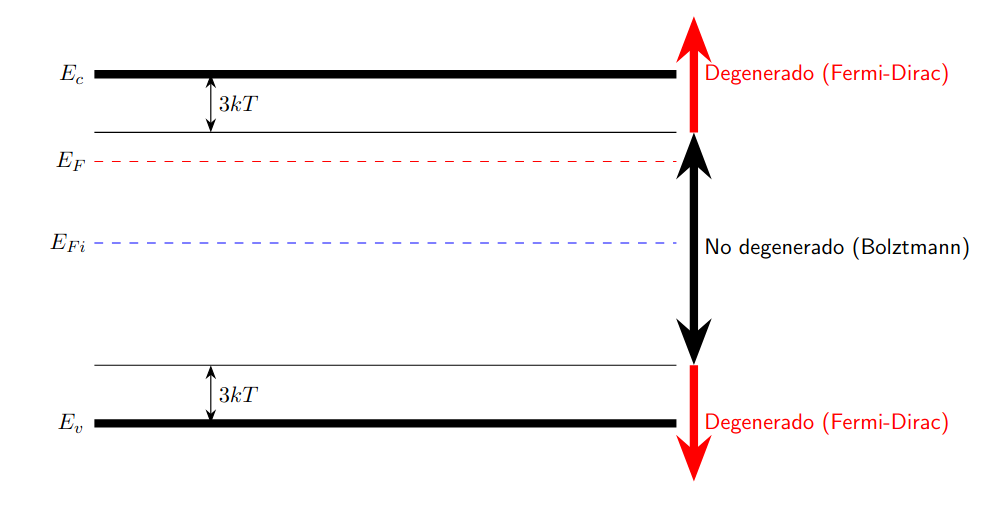
\includegraphics[width=0.85\textwidth]{Cuerpo/Ch_01/01_03.png}
	\caption{Régimen degenerado y no degenerado.}
\end{figure}


En general nosotros trabajaremos únicamente con semiconductores no degenerados, y por tanto en el rango de validez de la aproximación de Bolztmann, la que da como resultado las siguientes densidades de portadores:

\begin{equation}
	p=N_v e^{(E_v-E_F)/kT}  \qquad n = N_c e^{(E_F-E_c)/kT}
\end{equation}
donde $N_c$ y $N_v$ son las llamadas \textbf{densidades equivalentes de los estados de la banda de valencia y conducción}, con la siguiente forma:

\begin{equation}
	N_c = 2 \parentesis{\frac{m_n^* kT}{2\pi\hbar^2}}^{3/2} \tquad
	N_v = 2 \parentesis{\frac{m_p^* kT}{2\pi\hbar^2}}^{3/2}
\end{equation}
Para una temperatura aproximada de $300$K tenemos que

\begin{equation}
	N_{C,V} = (2.509\times10^{19} \cm^{-3}) \parentesis{\frac{m_{n,p}^*}{m_0}}^{3/2}
\end{equation}
siendo $m_0$ la masa del electrón.
\subsection{Semiconductores intrínsecos caso no degenerado}

Definimos como \textbf{semiconductor intrínseco} a un material semiconductor extremadamente puro, sin dopantes, cuyas propiedades solo dependan del material. En este tipo de materiales el número de electrones es igual al número de huecos (en virtud de la neutralidad electrónica: el número de electrones en la banda de conducción será el mismo el número que electrones faltan en la banda de valencia, i.e. el número de huecos). Matemáticamente se expresa como

\begin{equation}
	n = p = n_i
\end{equation}
y se llama \textit{condición intrínseca}. Siempre que estudiemos semiconductores intrínsecos lo haremos a través de los semiconductores no degenerados, ya que de cualquier otra forma no podemos tener expresiones analíticas. Denotamos $E_i$ al \textbf{nivel de fermi intrínseco}. Usando la ecuación anterior, obtenemos que:

\begin{equation}
	n_i = \sqrt{np} = \sqrt{N_CN_V} e^{-E_g/2kT} 
\end{equation}
donde $E_g=E_c-E_v$ y se le llama \textit{energía de gap}. El valor de $n_i$ para un semicdonductor dado es muy importante, incluso cuando está dopado. La razón es que siempre podemos expresar $n$ y $p$  en función de $n_i$ (a la misma temperatura), ya que si $n=p=n_i$:

\begin{equation*}
	n_i = N_C e^{(E_i-E_c)/kT} = N_V e^{(E_v-E_i)/kT}  \Rightarrow
\end{equation*}
\begin{equation}
	N_C=n_i e^{(E_c-E_i)/kT} \quad N_V = n_i e^{(E_i-E_v)/kT} \label{Ec:01-3-13}
\end{equation}
tal que
\begin{equation}
	n=n_i e^{(E_F-E_i)/kT} \qquad p = n_i e^{(E_i-E_F)/kT} \label{Ec:01-3-14}
\end{equation}
lo cual nos está dando en realidad una información muy relevante: en función del nivel de fermi, i.e., si $E_F>E_i$ o $E_F<E_i$, podremos saber si el conductor es de tipo $n$ o tipo $p$ (solo cuando $E_F=E_i$ tenemos $n=p$, precisamente la condición intrínseca). Además tenemos que de la expresión anterior podemos deducir la llamada \textbf{ley de acción de masas} (que se verifique siempre que estemos en el rango no degenerado):

\begin{equation}
	np=n_i^2
\end{equation}
Si nos damos cuenta a partir de las ecuaciones \ref{Ec:01-3-13} podemos deducir una \textit{expresión para la posición del nivel de Fermi intrínseco $E_i$}. Para esto partimos de las ecuaciones \ref{Ec:01-3-14}, de lo que se deduce que:

\begin{equation}
	E_i = \frac{E_c+E_v}{2} + \frac{kT}{2} \ln \parentesis{\frac{N_C}{N_V}} = \frac{E_c+E_v}{2} + \frac{3}{4} kT \ln \parentesis{\frac{m_p^*}{m_n^*}}
\end{equation}
Incluso podemos obtener la \textit{expresión para la posición del nivel de Fermi $E_F$} para el caso más general. Para esto partimos de las ecuaciones

\begin{equation}
	\ln \parentesis{\frac{n}{n_i}} = \frac{1}{kT} \parentesis{E_F-E_i} \Rightarrow E_F = E_i + kT \ln \parentesis{\frac{n}{n_i}}
\end{equation}
\begin{equation}
	\ln \parentesis{\frac{p}{n_i}} = \frac{1}{kT} \parentesis{E_i-E_F} \Rightarrow E_F = E_i - kT \ln \parentesis{\frac{p}{n_i}}
\end{equation}
Siendo expresiones completamente compatibles (si se verifica una se verifica la otra) además de que mantienen la relación citada antes entre el nivel de Fermi y el número de portadores huecos/electrón.

\subsection{Semiconductores extrínsecos caso no degenerado}

Definimos como \textbf{semiconductor extrínseco} o \textbf{semiconductor dopado} a un material semiconductor al que se le han insertado átomos de otro grupo. Pero antes es importante preguntarse por qué se incluyen estos átomos en nuestro semiconductor, y cuáles son sus ventajas. La respuesta todavía no podemos darla de manera muy profunda, sin embargo si podemos decir lo siguiente: a temperaturas ambiente, la cantidad de portadores tipo $n$ y tipo $p$ intrínsecas son muy bajas, y por tanto habrá una conductividad muy baja. Cuando dopamos un semiconductor no solo estamos aumentando el número de portadores de un tipo, estamos aumentando la conductividad. De hecho, al ser capaces de controlar el nivel de dopado, podemos elegir la conductividad arbitrariamente, pudiendo optimizar y controlar totalmente las propiedades eléctricas.

Así pues, tenemos dos tipos de dopantes, que además definiran el tipo de portador mayoritario que tendremos. Tenemos pues:

\begin{itemize}
	\item \textbf{Dopante dador}. Los dopantes dadores o dadores aportan electrones a la banda de conducción (por lo general son elementos del grupo V, aportando un electrón), lo que hará que el portador mayoritario sea el portador $n$. A la concentración de dadores la denotamos por $N_D$. Entre ellos encontramos el fósforo (P), el arsénico (As) y el antimonio (Sb).
	\item \textbf{Dopante aceptor}. Los dopantes aceptores o aceptores aportan heucos a la banda de valencia (por lo general son elementos del grupo III, aportando un hueco), lo que hará que el portador mayoritario sea el portador $p$. A la concentración de dadores la denotamos por $N_A$. Entre ellos encontramos el boro (B), el aluminio (Al) y el galio (Ga).
\end{itemize}

\begin{figure}[h!] \centering
	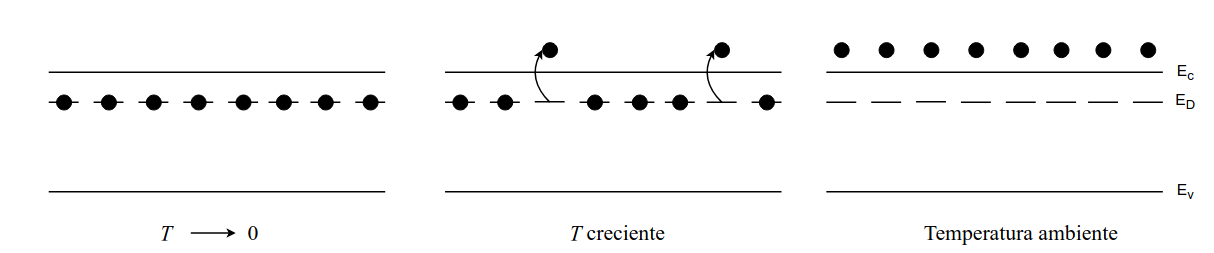
\includegraphics[width=0.9\textwidth]{Cuerpo/Ch_01/01_04.png}
	\caption{Funcionamiento de los conductores tipo $n$.}
\end{figure}

\begin{figure}[h!] \centering
	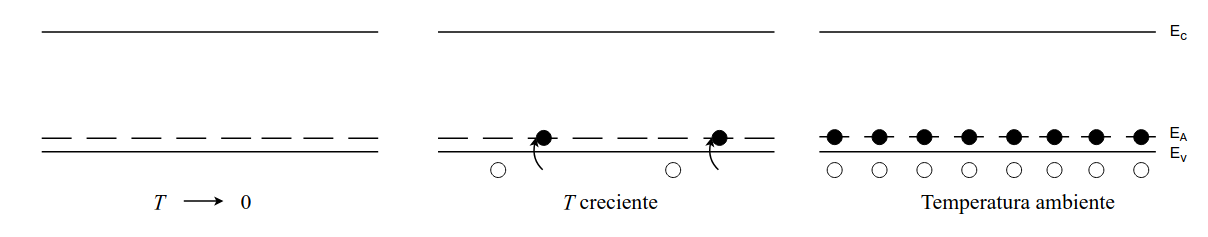
\includegraphics[width=0.9\textwidth]{Cuerpo/Ch_01/01_05.png}
	\caption{Funcionamiento de los conductores tipo $p$.}
\end{figure}

Sin embargo no es igual el número de impurezas $N_D$ y $N_A$ al número de portadores que aportan $N_D^+$ y $N_A^-$. Pensemos por ejemplo el caso de los elementos del grupo V. Para que puedan aportar el quinto electrón es necesario romper el enlace que lo une con dicho átomo, es decir, hace falta ionizarlo, lo que se hace a través de la aportación de energía, por ejemplo energía térmica. A partir de cierta temperatura todas las impurezas están ionizadas (temperatura ambiente). Sin embargo no siempre será así, y si la energía térmica no es suficiente para ionizar todas las impurezas, debemos usar las siguientes expresiones:

\begin{equation}
	N_D^+ = \frac{N_D}{1+g_D e^{(E_F-E_D)/kT}} \tquad
	N_A^- = \frac{N_A}{1+g_D e^{(E_A-E_F)/kT}}
\end{equation}
donde $E_D$ y $E_A$ son las correspondientes energías de ionización. Al igual que antes tenemos la condición de electroneutralidad, aunque ahora va a cambiar un poco: tenemos que considerar que $N_D^+$ y $N_A^-$ aportan carga. Así pues, la \textbf{condición de electroneutralidad para extrínsecos} es:

\begin{equation}
	p + N_D^+ = n + N_A^-
\end{equation}
lo cual tiene todo el sentido del mundo: si tenemos $N_D^+>N_A^-$ (mas dadores que aceptores) lógicamente habrá más portadores tipo $n$ que tipo $p$. Dado que la ley de acción de masas $np=n_i^2$ se cumple \textit{para cualquier semiconductor no degenerado}, para cualquier conductor no degenerado extrínseco podemos conocer $n$ y $p$ en función de $n_i,N_D^+$ y $N_A^-$ (que surge tras despejar una ecuación de segundo grado):

\begin{equation}
	n = \frac{N_D-N_A}{2} + \ccorchetes{\parentesis{\frac{N_D-N_A}{2}}^2 + n_i^2}^{1/2} \tquad p = \frac{N_A-N_D}{2} + \ccorchetes{\parentesis{\frac{N_A-N_D}{2}}^2 + n_i^2}^{1/2}
\end{equation}
Los 3 casos más sencillos que nos pueden plantear son los siguientes:

\begin{itemize}
	\item Cuando $N_D^+=N_A^-$ tenemos que
	      \begin{equation}
		      n=p=n_i
	      \end{equation}
	\item Cuando $N_D^+ \gg N_A^-,n_i$. En este caso tenemos las siguientes ecuaciones:
	      \begin{equation}
		      n=N_D^+ \tquad p = \frac{n_i^2}{N_D^+}
	      \end{equation}
	\item Cuando $N_A^-\gg N_D^+,n_i$. En este caso tenemos las siguientes ecuaciones:
	      \begin{equation}
		      p=N_A^- \tquad n = \frac{n_i^2}{N_A^-}
	      \end{equation}
\end{itemize}
El resto de casos habrá que calcularlos aparte.

\subsection{Semiconductores extrínsecos: régimen intrínseco y extríseco}

Definimos como \textbf{régimen extrínseco} de un semiconductor extrínseco\footnote{Muchas veces, cuando se dice que está en el semicdonductor está en el régimen extrínseco ya se asume que está dopado, y por tanto se obvia.} aquel intervalo de temperaturas (aunque puede ser otra variable) en el que todas las impurezas están ionizadas y se verifica que $N_D^+$ o $N_A^-$ es mucho mayor que $n_i$. Definimos como \textbf{régimen intrínseco} aquella región de temperaturas en la cual el nivel de impurezas excitadas es comparable o menor al número de portadores excitados por fluctuaciones térmicas $n_i$. Cuando la temperatura es baja y no están excitados todas las impurezas, decimos que estamos en el régimen de \textit{freeze out}.

Definimos como \textbf{temperatura intríseca} a la temperatura que separa el régimen extrínseco e intrínseco, y se define como aquella temperatura para la cual $n(T_i)=2N_D$ o $p(T_i)=2N_A$ en función de si es dador o aceptor el dopante.


\begin{figure}[h!] \centering
	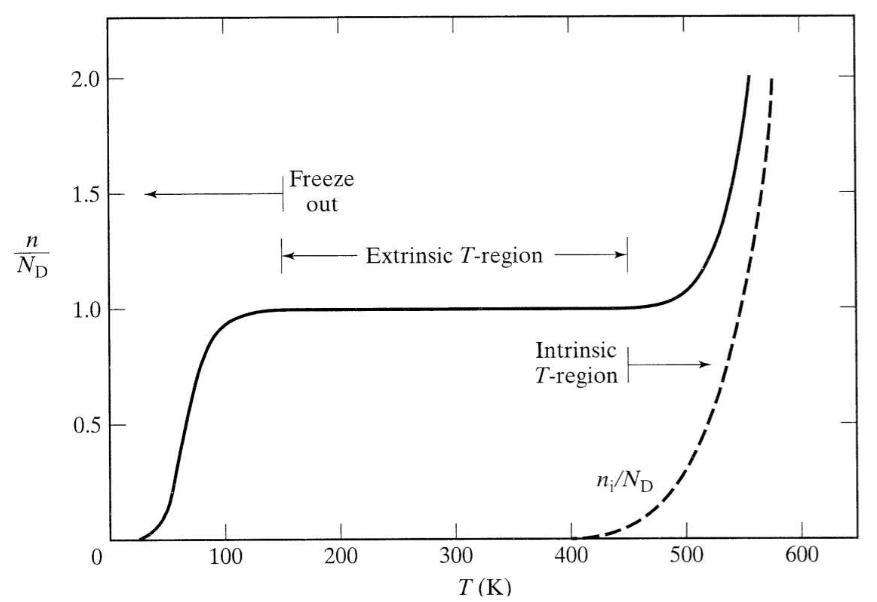
\includegraphics[width=0.85\textwidth]{Cuerpo/Ch_01/01_06.png}
	\caption{Régimenes intrínsecos y extrínsecos en función de la temperatura.}
\end{figure}


%%%%%%%%%%%%%%%%%%%%%%%%%%%%%%%%%%%%%%%%%%%%%%%%%%%%%%%%%%%%%%%%%%%%%%%
%%%%%%%%%%%%%%%%%%%%%%%%  SECCIÓN 4 %%%%%%%%%%%%%%%%%%%%%%%%%%%%%%%%%%%
%%%%%%%%%%%%%%%%%%%%%%%%%%%%%%%%%%%%%%%%%%%%%%%%%%%%%%%%%%%%%%%%%%%%%%%

%\section{Valores típicos}


\newpage


%%%%%%%%%%%%%%%%%%%%%%%%%%%%%%%%%%%%%%%%%%%%%%%%%%%%%%%%%%%%%%%%%%%%%%%
%%%%%%%%%%%%%%%%%%%%%%%%%%%%%%%%%%%%%%%%%%%%%%%%%%%%%%%%%%%%%%%%%%%%%%%
%%%%%%%%%%%%%%%%%%%%%%%%%%%%%%%%%%%%%%%%%%%%%%%%%%%%%%%%%%%%%%%%%%%%%%%
%%%%%%%%%%%%%%%%%%%%%%%%  EJERCICIOS %%%%%%%%%%%%%%%%%%%%%%%%%%%%%%%%%%
%%%%%%%%%%%%%%%%%%%%%%%%%%%%%%%%%%%%%%%%%%%%%%%%%%%%%%%%%%%%%%%%%%%%%%%
%%%%%%%%%%%%%%%%%%%%%%%%%%%%%%%%%%%%%%%%%%%%%%%%%%%%%%%%%%%%%%%%%%%%%%%
%%%%%%%%%%%%%%%%%%%%%%%%%%%%%%%%%%%%%%%%%%%%%%%%%%%%%%%%%%%%%%%%%%%%%%%

\section{Ejercicios}

\subsection{Ejercicio 1}


	Se dopa silicio con Boro (B) en una proporción de 2 ppm (partes por millón)
	\begin{enumerate}[label=\alph*)]
		\item Calcula la concentración intrínseca del Si y obten una expresión de dicha concentración en función de la temperatura.
		\item Indica el tipo de conducción de este material y calcula la concentración de impurezas y la de electrones y huecos (n y p) a temperatura ambiente si todos los dopantes están ionizados.
		\item Calcula la posición del nivel de Fermi y dibuja el diagrama de bandas completo correspondiente.
		\item ¿Qué pasa si la concentración de impurezas igualase el valor de \( N_V \)? Representa gráficamente las bandas de energía frente a la concentración de impurezas usando todas las aproximaciones que conozcas.
	\end{enumerate}
	(DATO: Constante de red del Si \( a_0 = 5.431 \) Å).


\rule{\textwidth}{0.1pt} \\[2pt]

	Veamos las soluciones por apartados
	\begin{enumerate}[label=\alph*)]
		\item La concentración intrínseca del Silicio en un semiconductor es el número de portadores $n_i$ en el semiconductor, si no estuviera dopado. No hay que confundir la concentración intrínseca $n_i$ con la concentración $n$, en la que si se tendrá en cuenta que el material está dopado. La concentración intrínseca es:

		      \begin{equation}
			      n_i = \sqrt{N_cN_v} e^{-E_G/2kT}
		      \end{equation}
		      donde $E_G=E_c-E-v$, y además

		      \begin{equation}
			      N_{C,V} = 2 \parentesis{\frac{m_{e,p}^* kT}{2\pi\hbar^2}}^{-3/2}
		      \end{equation}
		      Las masass $m_p^*= 1.18m_e$ y $m_n^*=0.81m_e$. Si queremos dar el valor:

		      \begin{equation}
			      N_c = 3.22 \cdot 10^{19} \cm^{-3} \tquad 	N_v = 1.83 \cdot 10^{19} \cm^{-3}
		      \end{equation}
		      De lo que se deduce

		      \begin{equation}
			      n_i = 9.56 \cdot 10^9 \cm^{-3}
		      \end{equation}


		\item Están dopando con boro, que es del grupo III, y por tanto es un dador. Esto significa que será un conductor tipo $p$. Para calcular la concentración de impurezas, primero tenemos que obtener la densidad de Boro en nuestro silicio. La densidad del silicio se calcular a partir de la constante de red y sabiendo que posee una red diamante. Así pues:
		      \begin{equation}
			      N_{Si} = \frac{8}{a_0^3}
		      \end{equation}
		      de lo que se puede deducir entonces que:
		      \begin{equation}
			      N_B = 2\cdot 10^{-6} \cdot N_{Si} = 9.988 \cdot 10^16 \cm^{-3}
		      \end{equation}
		      Nos dicen que todos los dopantes están ionizados, es decir, que estamos en el régimen extrínseco. En este régimen todos los átomos de Boro son impurezas, tal que $N_A^-=N_A=N_B$. Suponiendo que $N_A^- \gg N_D^+$, tenemos que la ecuación de neutralidad de carga:

		      \begin{equation}
			      n\cdot p = n_i^2 \tquad p-n-N_A = 0
		      \end{equation}
		      usando estas ecuaciones para despejar el valor de $n$ y $p$, tenemos que:
		      \begin{equation}
			      p = \frac{N_A}{2} + \ccorchetes{\parentesis{\frac{N_A}{2}}^2 + n_i^2}^{1/2}
		      \end{equation}
		      y luego calculamos

		      \begin{equation}
			      n = \frac{n_i^2}{p}
		      \end{equation}
		      Numéricamente podemos obtener los resultados:

		      \begin{equation}
			      n=915.034 \cm^{-3} \quad p = 9.988 \cdot 10^{16} \cm^3
		      \end{equation}


		\item La posición del nivel de Fermi de un semiconductor dopado se calcula a partir del nivel de Fermi intrínseco. Así pues
		      \begin{equation}
			      E_{Fi} = E_i = \frac{E_c+E_v}{2} + \frac{3 kT}{4} \ln \frac{m_p^*}{m_e^*} = 0.523 \text{eV}
		      \end{equation}
		      tal que la energía de Fermi. *Introducir imagen*
		      \begin{equation}
			      E_F = E_i + kT \ln \parentesis{\frac{p}{n_i}} = 0.135 \text{0.135}
		      \end{equation}
		\item Cuando la concentración de impurezas es igual al valor de $N_V$, dado que $p=N_V e^{(E_v-E_F)/kT}$, esto implicaría que $E_v = E_F$, y que por tanto la condición de \textit{semiconductor no degnerado} $E_F>E_v + 3kT$ no se cumpliría. \textit{Tenemos un semiconductor degenerado, teniendo que calcular los valores de $n$ y $p$ mediante las integrales explícitas}. Consecuentemente, estamos ante un semiconductor degenerado. *Introducir imagen para las bandas*.
	\end{enumerate}

\rule{\textwidth}{0.1pt} \\[2pt]

\subsection{Ejercicio 2}

	Una muestra de Si está dopada con \( 6 \times 10^{15} \) átomos de As por cm$^3$
	\begin{enumerate}[label=\alph*)]
		\item ¿Cuál es la concentración de portadores en la muestra de Si a 300 K?
		\item ¿Cuál es la concentración de portadores a 470 K?
		\item Para cada una de las dos temperaturas anteriores determinar la posición de \( E_i \), calcular \( E_F - E_i \) y dibujar a escala el diagrama de bandas de energía para la muestra.
		\item Si dopamos el Si con \( 10^{16} \) átomos donadores y \( 5 \times 10^{15} \) átomos aceptores por cm$^3$. ¿Cuál es la concentración de portadores a 300 K?+
		\item Partimos de una muestra de Si puro y lo dopamos exclusivamente con \( 10^{14} \) átomos donadores y \( 10^{14} \) átomos aceptores por cm³. Calcula la concentración de portadores y explica el resultado obtenido.
	\end{enumerate}
	Tener en cuenta que \( E_G = 1.08 \) eV a 470 K y suponer que \( m_e^*/m_h^* = 0.69 \) es independiente de la temperatura.


\rule{\textwidth}{0.1pt} \\[2pt]

	\begin{enumerate}[label=\alph*)]
		\item Tenemos primero que ver si está degenerado, sin embargo sabemos que para esta temperatura y el nivel de dopamiento no debería estar degenerado, y por tanto podríamos usar la ley de acción de masas junto con la condición de electroneutralidad para despejar $n$ en función de $N_D,N_A$ y $n_i$. Se puede obtener, dado que $N_D \gg n_i,N_A$, tenemos que

		      \begin{equation}
			      n\approx N_D = 6\cdot 10^{15} \cm^{-3} \tquad n\cdot p = n_i^2 \Rightarrow p = 1.67 \cdot 10^4 \cm^{-3}
		      \end{equation}
		\item Nos dicen que a $T=470$K y que $E_G=1.08$eV. Lo único que no cambio es $N_D$. Lógicamente el número de portadores intrínsecos $n_i$ cambia al aumentar la temperatura: a mayor energía térmica promocionan más electrones, mas electrones van a poder excitarse desde la banda de valencia. Calculamos $n_i$ a partir de
		      \begin{equation}
			      n_i = \sqrt{N_cN_v} e^{-E_g/2kT}
		      \end{equation}
		      Luego solo tenemos que hacer

		      \begin{equation}
			      N_{c,v} = 4.829\cdot 10^{15} T^{3/2} \parentesis{\frac{m_{n,p}^*}{m_e}}
		      \end{equation}
		      A esta temperatura tenemos entonces que:

		      \begin{equation}
			      N_c = 6.3 \cdot 10^{19} \cm^{-3} \quad N_v = 3.6 \cdot 10^{19} \cm^{-3}
		      \end{equation}
		      Y por tanto

		      \begin{equation}
			      n_i = 7.74 \cdot 10^{13} \cm^{-3}
		      \end{equation}
		      De lo que se deduce, de nuevo, aplicnado la ley de acción de masas:

		      \begin{equation}
			      n=6.001 \cdot 10^{15} \cm^{-3} \quad p = 9.98 \cdot 10^{11} \cm^{-3}
		      \end{equation}
		\item Determina la posción del nivel de Fermi intrínseco. Es secillo que:
		      \begin{equation}
			      E_i = \frac{E_c + E_v}{2} + \frac{3}{4} kT \ln \parentesis{\frac{m_p^*}{m_n^*}}
		      \end{equation}
		      Una vez tenemos $E_i$ para cada una de las temperaturas, calculamos la temperatura final
		      \begin{equation}
			      E_F = E_i + kT \ln \parentesis{\frac{n}{n_i}}
		      \end{equation}
		      *Introducir imagen*
		\item.
		\item
	\end{enumerate}
    
\begin{Anotacion}
    \textcolor{red}{\textbf{Falta por acabar}}
\end{Anotacion}

\rule{\textwidth}{0.1pt} \\[2pt]

\subsection{Ejercicio 3}

	Cuestiones sobre el nivel de Fermi:

	\begin{enumerate}[label=\alph*)]
		\item Calcular la temperatura \( T \) para que el nivel de Fermi de un cristal de Silicio tipo N con \( N_D = 10^{16} \) cm\(^{-3}\) quedara a una energía \( E_G/3 \) por debajo de la banda de conducción. Suponer que \( N_C \) y \( E_G \) son constantes con la temperatura e iguales a sus valores a temperatura ambiente. Y repetir para el caso de dopar con \( N_D = 10^{18} \) cm\(^{-3}\).

		\item En un semiconductor determinado, la probabilidad de que los electrones ocupen un estado de energía \( kT \), por encima del extremo inferior de la banda de conducción es \( e^{-10} \). Determinar la posición del nivel de Fermi en dicho material.

		\item ¿Cuál es la probabilidad de que un estado de energía \( kT \) por debajo del nivel de Fermi esté ocupado por un hueco?
	\end{enumerate}

\rule{\textwidth}{0.1pt} \\[2pt]


	\begin{enumerate}[label=\alph*)]
		\item La solución es $T=536.206$K. Para esto tenemos que usar la relación
		      \begin{equation}
			      T = \frac{E_F-E_c}{k} \frac{1}{\ln (N_D/N_c)} =  \frac{-E_g}{3k} \frac{1}{\ln (N_D/N_c)}
		      \end{equation}
		      donde $N_c=3.22\cdot 10^{19}\cm^{-3}$.
		\item Queremos calcular la posición del nivel de Fermi. Usamos la fórmula
		      \begin{equation}
			      f(E) = \frac{1}{1+e^{(E-E_F)/kT}}
		      \end{equation}
		      y usando lo que nos da el enunciado:
		      \begin{equation}
			      f(kT+E_c) = \frac{1}{1+e^{(kT+E_c-E_F)/kT}}
			      = \frac{1}{e^{10}}
		      \end{equation}
		      Tenemos entonces que

		      \begin{equation}
			      1+e^{\frac{kT+E_c-E_f}{kT}} = e^{10}
		      \end{equation}
		      De lo que se deduce que $E_F = E_c + 9kT$.
		\item ¿Cuál es la probabilidad de que un estado de energía \( kT \) por debajo del nivel de Fermi esté ocupado por un hueco? Tenemos que
		      \begin{equation}
			      1-f(E_F-kT) = 1 - \frac{1}{1+e^{-1}} \simeq 0.2689 \rightarrow 26.89 \%
		      \end{equation}
		      La probabilidad es no nula y por tanto... (preguntar a Elisa Casal).
	\end{enumerate}

\rule{\textwidth}{0.1pt} \\[2pt]

\subsection{Ejercicio 4}

Responde a las siguientes cuestiones:
\begin{enumerate}
	\item[a)] A 300 K la densidad efectiva de estados en la banda de valencia es $1.83 \times 10^{19} \text{ cm}^{-3}$ para el silicio y $9.0 \times 10^{18} \text{ cm}^{-3}$ para el GaAs. Calcular sus correspondientes masas efectivas para los huecos. Comparar estas masas con la masa del electrón en el vacío.

	\item[b)] Calcula y representa la posición del nivel intrínseco en silicio a temperatura ambiente y a 1000 $^{\circ}$C (tomamos $m_p = 1.0m_0$ y $m_n = 0.19m_0$), asumiendo que el gap se mantiene constante. ¿Es razonable asumir que $E_i$ se encuentra en la mitad de la banda prohibida?
\end{enumerate}

\rule{\textwidth}{0.1pt} \\[2pt]


\begin{enumerate}[label=\alph*)]
	\item	Tenemos que calcular la masa efectiva de los huecos para dos semiconductores diferentes, dado su densidad efectiva de estados en la banda de valencia. Esto significa que necesitamos invertir la fórmula típica, tal que
		  \begin{equation}
			  N_V = 2 \parentesis{\frac{m_p^* kT}{2\pi\hbar^2}}^{3/2} \quad \Rightarrow \quad m_p^* = \parentesis{\frac{N_V}{2}}^{2/3} {\frac{2 \pi \hbar^2}{kT}}
		  \end{equation}
		  De lo que se deduce que para el Si y el GsAs:

		  \begin{equation}
			  \text{Si:} \quad m_p^* = 7.38\cdot10^{-31} \text{kg} = 0.81 \ {m}_e
		  \end{equation}
		  \begin{equation}
			  \text{GaSi:}\quad m_p^* = 4.59 \cdot10^{-31} \text{kg} = 0.51 \ {m}_e
		  \end{equation}
		  Nivel intríseco 300K 1.7505319217070854
	\item Tenemos que calcular la posición del nivel intrínseco $E_i$ a la temperatura ambiente (300 K) y a 1000 $^\circ C$, asumiendo que $E_g$ es constante. Veamos que solo es aplicar una fórmula:
		  \begin{equation}
			  E_i = \frac{E_c+E_v}{2} + \frac{3}{4} kT \ln\parentesis{\frac{m_p^*}{m_n^*}}
		  \end{equation}
		  donde hemos considerado que $E_g=1.12$ en el silicio, y que $E_v=0$, ergo $E_c=1.12$. Hacemos la representación gráficamente. Las energías son: $300K: \ E_i=0.57$ eV y a 1273K $E_i: 0.70$ eV. Las masas usadas a 300K son: $m_p=0.81m_e$ y $m_n=1.18m_e$.
		  \begin{center}
			  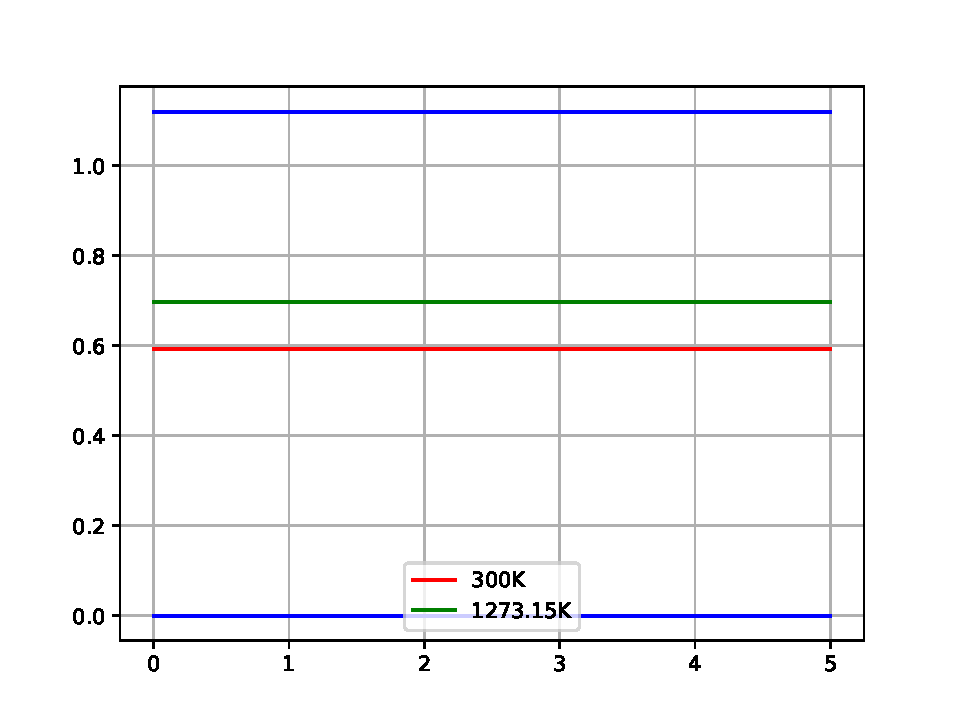
\includegraphics[width=0.6\textwidth]{Cuerpo/Ch_01/Ejercicio_01_5.pdf}
		  \end{center}
		  Viendo esta imagén no parece descabellado consdierar $E_i$ constante.
\end{enumerate}


\rule{\textwidth}{0.1pt} \\[2pt]

\subsection{Ejercicio 5}

\begin{enumerate}[label=\alph*)]
	\item En GaN a 300 K, $E_G = 3.43$ eV, $m_n^*/m_0 = 0.2$, $m_p^*/m_0 = 1.25$ y $n_i = 1.37 \times 10^{-10} \text{ cm}^{-3}$. Explicar cualitativamente (sin utilizar la fórmula que calcula el valor de $E_i$) si el nivel de Fermi intrínseco en InSb estará más próximo a la $E_C$ o a la $E_V$. Comprobarlo a continuación usando la fórmula.

	\item Las distribuciones de portadores, o número de portadores en función de la energía en las bandas de conducción y de valencia presentan un máximo a una energía próxima a los bordes de las bandas. Considerando el semiconductor como no degenerado, calcular la energía a la que se encuentra el máximo en la distribución de electrones.
\end{enumerate}

\rule{\textwidth}{0.1pt} \\[2pt]


\begin{enumerate}[label=\alph*)]
	\item El nivel de Fermi intrínseco a temperatura no nula está mas cerca de $E_c$ si la masa efectiva de los huecos es mayor que la masa efectiva de los electrones, y más cerca de $E_v$ si la masa de los electrones es mas grande que la de los huecos. ¿Por qué? Como sabemos, la masa efectiva de los electrones/huecos es inversamente proporcional a la curvatura en el mínimo/máximo de la banda de conducción/valencia. Cuanto mayor sea la curvatura, mas energía se tiene que darse para ocupar la misma cantidad de estados. Como consecuencia, la energía de fermi intríseca, que se define como la mitad del valor entre $E_c$ y $E_v$ tendría que tirar hacia la banda con más curvatura, i.e. la que tiene menos masa efectiva. \textcolor{BrickRed}{Francamente no me tiene mucho sentido, ya que $E_c$ y $E_v$ no debería cambiar. Existen otras formas de verlo a través de la función de Fermi y la densidad de estados, habría que investigarlo.}

	En nuestro caso esto implica que \textit{debería estár mas cerca de la banda de conducción}. Para los valores dados, tenemos que

	\begin{equation}
		  E_i = \frac{E_c+E_v}{2} + \frac{3}{4} kT \ln\parentesis{\frac{m_p^*}{m_n^*}} = 1.75 \ \text{eV}
	\end{equation}
	que considerando $E_v=0$ y $E_c=E_g=3.43$ eV vemos que está mas cerca de la banda de conducción $E_c$ que de $E_v$.
	\item La concentración de electrones en la banda de conducción está dada por:

		  \[
			  n(E) = g_c(E) f(E)
		  \]

		  donde

		  \begin{itemize}
			  \item La densidad de estados en la banda de conducción es:

					\[
						g_c(E) = \frac{8\pi \sqrt{2} m_c^{3/2}}{h^3} (E - E_c)^{1/2}
					\]

			  \item La función de distribución de Fermi-Dirac en la aproximación no degenerada (Maxwell-Boltzmann) es:

					\[
						f(E) \approx e^{-\frac{(E - E_F)}{k_B T}}
					\]
		  \end{itemize}

		  Por lo que la distribución de portadores en la banda de conducción es:

		  \[
			  n(E) = \frac{8\pi \sqrt{2} m_c^{3/2}}{h^3} (E - E_c)^{1/2} e^{-\frac{(E - E_F)}{k_B T}}
		  \]

		  Para encontrar el máximo, derivamos respecto a \( E \) e igualamos a cero:

		  \[
			  \frac{d}{dE} \left[ (E - E_c)^{1/2} e^{-\frac{(E - E_F)}{k_B T}} \right] = 0
		  \]

		  Aplicando la regla del producto:

		  \[
			  \frac{1}{2} (E - E_c)^{-1/2} e^{-\frac{(E - E_F)}{k_B T}} + (E - E_c)^{1/2} e^{-\frac{(E - E_F)}{k_B T}} \left(-\frac{1}{k_B T} \right) = 0
		  \]

		  Factorizando:

		  \[
			  e^{-\frac{(E - E_F)}{k_B T}} (E - E_c)^{-1/2} \left[ \frac{1}{2} - \frac{(E - E_c)}{k_B T} \right] = 0
		  \]

		  Para que se cumpla la igualdad, la expresión entre corchetes debe ser cero:

		  \[
			  \frac{1}{2} = \frac{(E - E_c)}{k_B T}
		  \]

		  Despejando \( E \):

		  \[
			  E - E_c = \frac{1}{2} k_B T
		  \]
		  Por lo tanto, el máximo de la distribución de electrones en la banda de conducción se encuentra a:

		  \[
			  E_{\text{max}, c} = E_c + \frac{1}{2} k_B T
		  \]

		  Siguiendo el mismo procedimiento para los huecos en la banda de valencia:

		  \[
			  E_{\text{max}, v} = E_v - \frac{1}{2} k_B T
		  \]

		  Esto significa que los portadores tienden a concentrarse en energías lige,amente por encima del borde de la banda de conducción y por debajo del borde de la banda de valencia en aproximadamente \( \frac{1}{2} k_B T \). El doctorando hizo un dibujo que dijo que sale en el Pierret, sobre la multiplicación de producto de la densidad de estados y las bandas. Véase notas a mano.

\end{enumerate}


\rule{\textwidth}{0.1pt} \\[2pt]

\subsection{Ejercicio 6}

Dibujar un diagrama de bandas para el silicio dopado con $10^{17}$ átomos/cm$^3$ de arsénico a 300 K y 600 K. Mostrar el nivel de Fermi, $E_C$, $E_V$ y utilizar el nivel de Fermi intrínseco como energía de referencia, asumiendo el caso de ionización total. La variación del bandgap con la temperatura viene dada por la expresión de Varshni (DOI: 10.1016/0031-8914(67)90062-6):

\begin{equation}
	E_G(T) = E_G(0) - \frac{\alpha T^2}{T + \beta}
\end{equation}

Para el silicio $\alpha = 4.73 \times 10^{-4} \text{ eV/K}$, $\beta = 636 \text{ K}$ y $E_G(0) = 1.17 \text{ eV}$. Suponer que las masas efectivas se mantienen constantes con la temperatura.



\rule{\textwidth}{0.1pt} \\[2pt]


Nos dicen que dibujemos un diagrama de bandas para el silicio dopado por arsénico (grupo V, dador) completamente ionizado. Esto implica necesariamente calcular $E_i,E_c,E_v$ y $E_F$. Primero vamos a despejar $E_i$ y $E_v$, luego despejaremos en función de estos $E_F$. Recordar que

\begin{equation}
	E_i = \frac{E_v+E_c}{2} - \frac{3}{4} kT \ln\parentesis{\frac{m_n^*}{m_p^*}}
\end{equation}

\begin{itemize}
	\item Como hemos dicho despejamos estas energías. Dado que $E_i$ es nuestra referencia, las ecuaciones a usar son, a una $T$ dada, que:
		  \begin{equation}
			  E_c-E_v = E_g(0) - \frac{\alpha T^2}{T+\beta} \qquad E_c+E_v=-2 \cdot \frac{3}{4} kT\ln \parentesis{\frac{m_n^*}{m_p^*}}
		  \end{equation}
		  De lo cual se deduce que:
		  \begin{equation}
			  E_c = \frac{1}{2} \ccorchetes{E_g(0) - \frac{\alpha T^2}{T+\beta} - \frac{3}{2} kT^{3/2} \ln \parentesis{\frac{m_n^*}{m_p^*}}}
		  \end{equation}
		  \begin{equation}
			  E_v = \frac{1}{2} \ccorchetes{-E_g(0) +\frac{\alpha T^2}{T+\beta} - \frac{3}{2} kT^{3/2} \ln \parentesis{\frac{m_n^*}{m_p^*}}}
		  \end{equation}
		  Usando las masas de portadores $m_n^*=1.18m_e$ y $m_p^*=0.81m_e$  (y considerado, como nos dice el enunciado, que son constantes frente a la tempratura). Obteniendo los siguientes resultados numéricos:
		  \begin{equation}
			  \text{300K}: \qquad
			  E_c = 0.570 \ \text{eV} \quad E_v = -0.554 \ \text{eV}
		  \end{equation}
		  \begin{equation}
			  \text{600K}: \qquad
			  E_c = 0.531  \ \text{eV} \quad E_v = -0.502\ \text{eV}
		  \end{equation}
	\item Ahora tenemos que calcular $E_F$, que viene dado, en un conductor dopado $N$ no degnerado por (recordar que $E_i=0$)
		  \begin{equation}
			  E_F = kT \ln \parentesis{\frac{N_D}{n_i}}
		  \end{equation}
		  Dado que conocemos $T$ y $N_D$, solo resta saber el valor de $n_i$, para lo cual hemos usado la expresión:

		  \begin{equation}
			  n_i = \sqrt{N_c N_v} e^{-E_g/2kT}
		  \end{equation}
		  siendo $N_c$ y $N_v$ las típicas funciones que dependen de la masa efectiva y del a temperatura. Así pues, obtenemo los resultados:
		  \begin{equation}
			  \text{300K:}\quad
			  E_F = 0.420 \ \text{eV} \qquad
			  \text{600K:}\quad
			  E_F= 0.178 \ \text{eV}
		  \end{equation}
\end{itemize}
Una vez tenemos esto podemos realizar la representación:
\begin{center}
	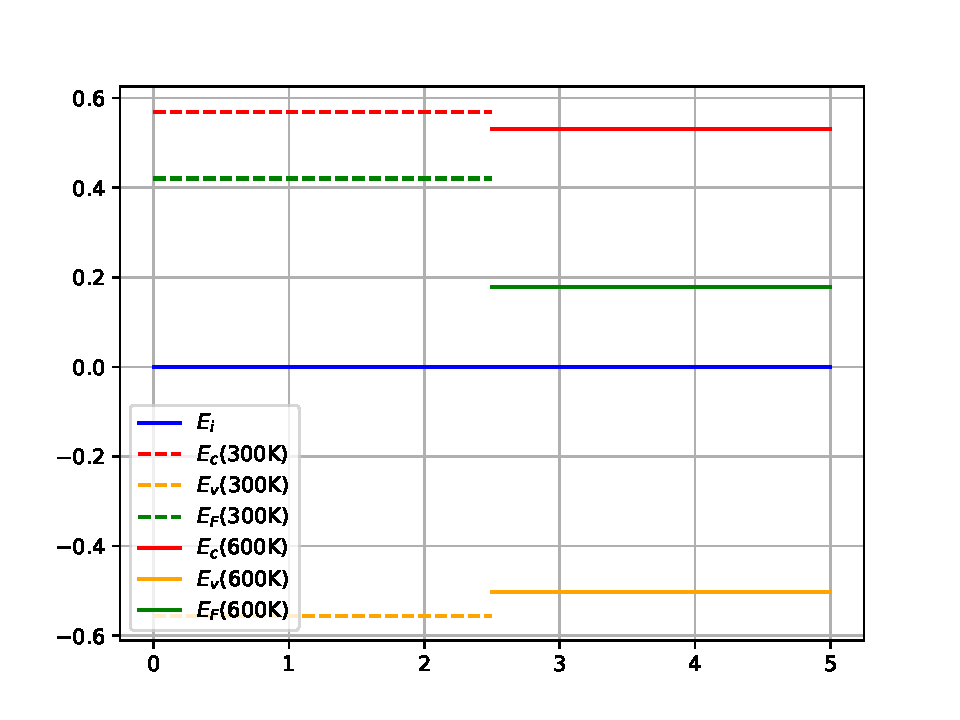
\includegraphics[width=0.9\linewidth]{Cuerpo/Ch_01/Ejercicio_01_7.pdf}
\end{center}


\rule{\textwidth}{0.1pt} \\[2pt]

\subsection{Ejercicio 7}

Calcular el nivel de Fermi y dibujar el diagrama de bandas completo de silicio dopado con $10^{15}$, $10^{17}$ y $10^{19}$ átomos/cm$^3$ de P ($E_D = 0.045$ eV) a temperatura ambiente suponiendo ionización total de las impurezas. A partir del nivel de Fermi calculado comprobar si esta suposición es correcta para cada valor de dopado. Asumir que los átomos donadores ionizados vienen dados por la expresión:

\begin{equation}
	N_D^+ = \frac{N_D}{1 + 2 \exp \left( \frac{E_F - E_D}{kT} \right)}
\end{equation}

\rule{\textwidth}{0.1pt} \\[2pt]

La solución del ejercicio pasa por calcular los valores de los niveles de Fermi usando la ecuación
\begin{equation}
	E_F = E_i + kT \ln \parentesis{\frac{N_D}{n_i}}
\end{equation}
Recordemos que en este caso definimos $E_{c}=0$ eV. Consecuentemente tanto $E_D$ como $E_F$ serán negativos. Estamos ante un dador que tiene todos los átomos excitados $N_D$ tal que $N_D>>n_i,N_A$. Dado que consideramos esto a tempeartura ambiente, tenemos que $n_i=1.18\cdot 10^{10} \ \cm^{-3}$ y por tanto que para estos $N_D$:
\begin{equation}
	N_D=10^{15} \ \cm^{-3} \Rightarrow E_F = -0.27 \ \eV
\end{equation}
\begin{equation}
	N_D=10^{17} \ \cm^{-3} \Rightarrow E_F = -0.15  \ \eV
\end{equation}
\begin{equation}
	N_D=10^{19} \ \cm^{-3} \Rightarrow E_F = -0.035  \eV
\end{equation}
Una vez tenemos estos valores de $E_F$, veamos si es válido asumir que todosl os átomos donadores están ionizados, usando que

\begin{equation}
	N_D^+ = \frac{N_D}{1+2\exp\ccorchetes{(E_F-E_D)kT}}
\end{equation}
Tal que para las energías dadas:
\begin{equation}
	E_F= -0.27  \ \eV \Rightarrow N_D^+ =  9.999\cdot 10^{14}  \ \cm^{-3}
\end{equation}
\begin{equation}
	E_F = -0.15 \ \eV\Rightarrow N_D^+ =  9.722\cdot 10^{16} \ \cm^{-3}
\end{equation}
\begin{equation}
	E_F =-0.034 \ \eV \Rightarrow N_D^+ = 2.597 \cdot 10^{18}  \ \cm^{-3}
\end{equation}
Dibujamos los gráficos
\begin{center}
	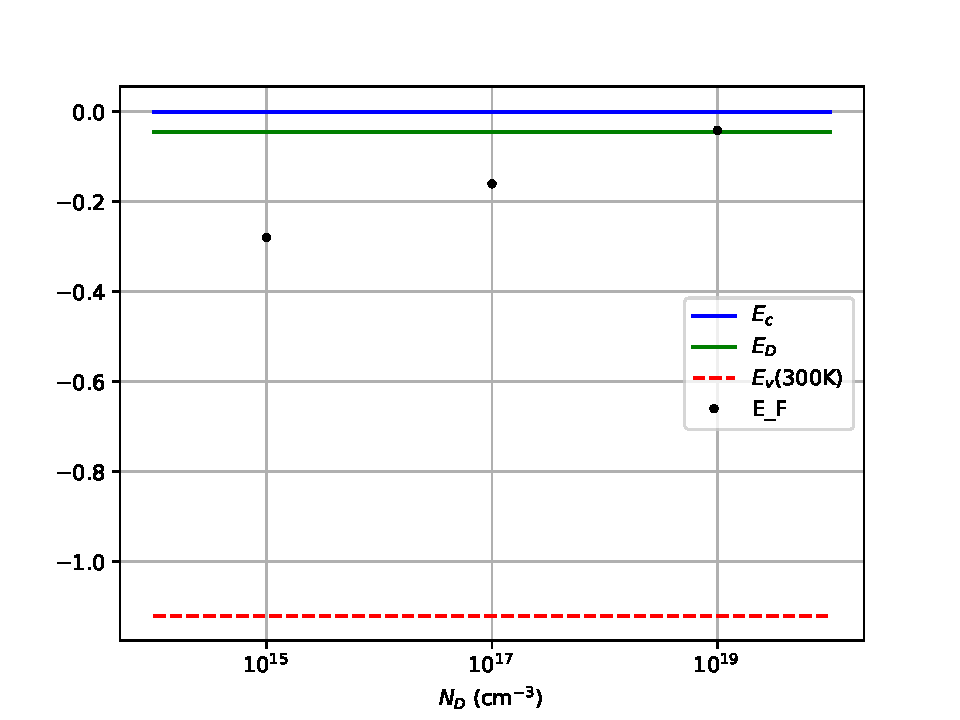
\includegraphics[width=0.9\linewidth]{Cuerpo/Ch_01/Ejercicio_01_8.pdf}
\end{center}



\rule{\textwidth}{0.1pt} \\[2pt]

\subsection{Ejercicio 8}

Responde a las siguientes cuestiones:

\begin{enumerate}
	\item[a)] Utilizando la expresión para los átomos donadores ionizados dada en el ejercicio anterior, calcular la concentración de donadores sin ionizar para una muestra de silicio dopada con $10^{16}$ átomos/cm$^3$ de P ($E_D = 0.045$ eV) a una temperatura de 50 K. El nivel de Fermi está situado a 0.0459 eV por debajo de la banda de conducción.

	\item[b)] Una muestra de silicio a $T = 300$ K contiene una concentración de impurezas aceptoras $N_A = 10^{16}$ cm$^{-3}$. Determinar la concentración de átomos donantes que debe ser añadida para que el silicio sea tipo N y la energía de Fermi esté 0.25 eV por debajo del borde de la banda de conducción.
\end{enumerate}


\rule{\textwidth}{0.1pt} \\[2pt]




